\documentclass[a4paper,12pt]{article}
%\documentclass[a4paper,10pt]{scrartcl}

\usepackage{amsmath,amssymb}
\usepackage{epic}
\usepackage{eepic}
\usepackage{bm}
\usepackage{array}
\usepackage{float}
\usepackage{multirow}
\usepackage{fancyhdr}

\usepackage{vmargin}            % red�finir les marges
\usepackage{amsthm}
\usepackage{graphicx,color}


\setmarginsrb{2cm}{0.5cm}{2cm}{1cm}{0cm}{1cm}{0cm}{1cm}
\newtheorem{remark}{Remark}

\newcommand{\normL}[1]{%
\ensuremath{||#1||_{L^2}}}
\newcommand{\normLL}[1]{%
\ensuremath{||#1||_{L^1}}}

\newcommand{\abs}[1]{%
\ensuremath{|#1|}}


\newcommand{\norme}[2]{%
\ensuremath{||#1||_{#2}}}

\renewcommand{\d}[0]{%
\ensuremath{\text{d}}}


\newcommand{\systeme}[1]{%
\ensuremath{\begin{numcases} \quad #1 \end{numcases}}}


\newcommand{\integ}[3]{%
\ensuremath{\displaystyle{\int^{#2}_{#1} #3}}}

\newcommand{\somme}[3]{%
\ensuremath{\displaystyle{\sum^{#2}_{#1} #3 }}}

\newlength{\intwidth}
\DeclareRobustCommand{\fpint}[2]
   {\mathop{%
      \text{%
        \settowidth{\intwidth}{$\int$}%
        \makebox[0pt][l]{\makebox[\intwidth]{$-$}}%
        $\int_{#1}^{#2}$}}}


\title{Potential Flow Around a Regular Body in 2D}
\author{}
\date{}

\begin{document}
\maketitle
\section{Setting of the Problem}

Suppose the fluid flow is described by velocity vector field $u$. The velocity field can be written as the gradient 
of a velocity potential $\phi$. 
\begin{equation}\label{Pr0}
 u=\nabla \phi
\end{equation}

Let us assume that the vector field $u$ is irrotational. It means 
$\text{curl}(u)=0$. We can also write
$\nabla\times u=0$.
Furthermore, we consider the flow to be incompressible, we have $\nabla\cdot u=0$. If we substitute \eqref{Pr0}, we have
\begin{align}
&\nabla \cdot u=0 \\
 &\nabla \cdot \nabla\phi=0 \\
 &\Delta \phi=0 \label{Pr1}
\end{align}

Let us consider a fluid in an infinite domain. Let us add a regular obstacle $\Omega_0$. We consider $\partial\Omega_0$ to be $C^1$. It means the obstacle doesn't have any angles nor discontinuities. 
On the border of the obstacle, the velocity is tangential.
\begin{equation}\label{eq1}
u\cdot n=0
\end{equation}
with $n$ is the (exterior) normal vector of $\Omega_0$.
We substitute \eqref{Pr0} to~\eqref{eq1}, we get 
\begin{equation}\label{Pr3}
\nabla\phi\cdot n=0
\end{equation}
Equation~\eqref{Pr3} is called an homogeneous Neumann boundary condition.  

Far from the obstacle, we suppose that the velocity is uniform. Without loss of generality, 
we assume that its direction is $\vec{e_x}$. 
This condition can be written as
\begin{equation} \label{Pr2}
u=u_0\vec{e_x} \quad \text{as }|x|\to\infty, |y|\to\infty
\end{equation}
We ilustrate our setting of problem in Figure \ref{settingOfProblem}.
\begin{figure}[!htbp]
\begin{center}
\includegraphics[height = 6cm]{settingOfProblem.eps}
\end{center}
 \caption{Geometry of the problem}\label{settingOfProblem}
\end{figure}

From \eqref{Pr1} and \eqref{Pr2}, we obtain the system:
\begin{align} \label{problem1}
\Delta \phi &=0\\
u=\nabla \phi &\to u_0 \vec{e_x} \quad \text{as } x\to\pm\infty
\end{align}
Without any obstacle, this problem has the obvious solution i.e $\phi= u_0 x$. If there exist a regular obstacle, we have to add a homogeneous Neumann boundary condition as in \eqref{Pr3}.
Then, we obtain the potential flow problem around a regular obstacle as follows:
\begin{align} \label{problem2}
\Delta \phi=0 \quad \text{On: } \mathbb{R}^2 \setminus \overline{\Omega_0}=\Omega\\
u=\nabla\phi\to u_0\vec{e_x}\quad \text{as } x \to \pm\infty\\
\nabla\phi \cdot n=0 \quad \partial \Omega_0=\Gamma_0
\end{align}
The problem is hence to find the harmonic function that satisfies all the boundary conditions.

Without the obstacle, problem \eqref{problem1} has solution $u_0x$. We can use it to find $\phi$. Let us perform a change of variable in order to get the solution of problem~\eqref{problem2}.
Let us define 
\begin{equation}
\psi=\phi-u_0 x \label{changevar} 
\end{equation}
If we substitute~\eqref{changevar} to the problem~\eqref{problem2} we can obtain as follows:
\begin{align}
 \Delta \psi &= \Delta \phi-\Delta (u_0x)\\
\Delta \psi &= \Delta \phi\\
\nabla \psi &= \nabla\phi-u_0\vec{e_x}
\end{align}
when $x\to\pm\infty$ value of $\nabla \psi\to 0$.
From here, we get 
\begin{equation}
 \nabla\psi\to0 \quad \text{as } x\to\pm\infty
\end{equation}
From the last condition in~\eqref{problem2} we get
\begin{align} 
\nabla\psi\cdot n &= \nabla(\phi-u_0 x)\cdot n \text{on } \Gamma_0\\
&=\nabla\phi \cdot n - \nabla(u_0 x)\cdot n\\
&=0-u_0\nabla x\cdot n\\
&=-u_0 \vec{e_x} \cdot n\\
&=-u_0 n_x
\end{align}

The problem become, after changing variable:
\begin{align}  \label{problem3}
\Delta \psi=0 \quad \text{in } \Omega\\
\nabla\psi \to 0 \quad \text{as } x\to\pm\infty\\
\nabla\psi \cdot n = -u_0 n_x \quad \text{on } \Gamma_0 
\end{align}
Once we solved the problem, if we want to retreive the velocity field, we simply compute:
\begin{align}
 u=\nabla\phi=\nabla(\psi+u_0 x)\\
= \nabla\psi+u_0 \vec{e}_x
\end{align}
\begin{remark}
 Uniqueness of solution problem ~\eqref{problem3} is not ensured. If $\psi$ is a solution of ~\eqref{problem3} then
$\Tilde{\psi} = \psi+const$ is also a solution. This is not really a physical problem, because the only thing that
matters to us is $\nabla\psi$. 
\begin{equation}
 \nabla \psi=\nabla\Tilde{\psi}
\end{equation}
\end{remark}
From here we get the actual problem is
\begin{align}  \label{problem4}
\Delta \psi=0 \quad \text{in } \Omega\\
\nabla\psi \to 0 \quad \text{as } x\to\pm\infty ?\\
\nabla\psi \cdot n = -u_0 n_x \quad \text{on } \Gamma_0 
\end{align}

\begin{remark}
 We didn't proof the existence and uniqueness solution of the ~\eqref{problem4} nor their regularity. We assume that 
the problem has all things we need.
In order to obtain the uniqueness, we will have to set the constant?, which will be done by selecting a particular Green function.
\end{remark}

\section{The Boundary Integral Equation}

Let $G_{x',y'} (x,y)$ be the Green function of Laplacian problem 2D.
\begin{equation} \label{GreenFunction}
 G_{x',y'}(x,y)=\dfrac{1}{2 \pi} \, \ln(\sqrt{(x-x')^2+(y-y')^2})
\end{equation}
$G$ has some properties:
\begin{align}
 \Delta G_{x',y'}=\delta_{x',y'}\\
 \nabla G_{x',y'}\to0\quad \text{at}\quad (x,y)\to\pm \infty
\end{align}

Let we us examine the problem:
\begin{align}  \label{problem5}
\Delta \psi=0 \quad \text{in } \Omega\\
\psi \to 0 \quad \text{as } x\to\pm\infty\\
\nabla\psi \cdot n = -u_0 n_x \quad \text{on } \Gamma_0 
\end{align}
If we multiply the first equation in~\eqref{problem5} with $G_{x',y'}$ and integrate over 
$\Omega$. By integrating by parts, we get:
\begin{align}
\Delta\psi=0\\
\Rightarrow&\integ{\Omega}{}{ \Delta \psi G_{x',y'}}=0\\
\Rightarrow& \integ{\Gamma_0}{}{(\nabla \psi \cdot n)G_{x',y'}}-\integ{\Omega}{}
{\nabla\psi \nabla G_{x',y'}}=0\\
\Rightarrow&\integ{\Gamma_0}{}{(\nabla \psi \cdot n)G_{x',y'}}-
\left\{\integ{\Gamma_0}{}{\psi \nabla G_{x',y'}\cdot n}-
\integ{\Omega}{}{\Delta G_{x',y'} \psi}\right\}=0 \label{int1}
\end{align}
let we postpone the result of~\eqref{int1} until these few remarks.
\begin{remark}
 If $(x',y')\in \Omega=\mathbb{R}^2 \setminus\overline{\Omega_0}$, then we obtain the following results:
\begin{enumerate}
 \item By using boundary condition
\begin{align}
 \integ{\Gamma_0}{}{\psi \nabla G_{x',y'}(x,y)\cdot n \, ds}&=\integ{\Gamma_0}{}{-u_0 n_x G_{x',y'} \, ds}\\
&= -u_0 \integ{\Gamma_0}{}{n_x G_{x',y'} \, ds}
\end{align}
\item By definition of Green function and dirac distribution
\begin{align}
 \integ{\mathbb{R}^2 \setminus \overline{\Omega_0}}{}{\Delta G_{x',y'} \psi }&=
{\langle\delta_{x',y'}{,} \psi\rangle}_{D',D}\\
&=\psi_{x',y'}
\end{align}
\end{enumerate}
\end{remark}
From these remarks, we can sum up the equation~\eqref{int1} 
when $(x',y')\in\mathbb{R}^2\setminus\overline{\Omega_0}$, not in boundary as
\begin{align}
 -u_0 \integ{\Gamma_0}{}{n_x G_{x',y'}(x,y) \, ds}-
\integ{\Gamma_0}{}{\psi\nabla G_{x',y'}(x,y)\cdot \vec{n} \, ds}+\psi(x',y')=0\\
\psi(x',y')=-\integ{\Gamma_0}{}{-u_0 n_x G_{x',y'}(x,y) -\psi\nabla G_{x',y'}(x,y)\cdot \vec{n} \, ds} \label{BIform}
\end{align}
We call equation~\eqref{BIform} as Boundary Integral Formulation in $(x',y')\in \mathbb{R}^2\setminus\overline{\Omega_0}$. From boundary integral formulation we can see that the potential in 
every point in domain is depend on its potential and gradient of potential on the boundary.

We want to compute $\psi$ on the boundary. In order to obtain a closed integral equation, we want to evaluate $\psi(x',y')$
when $(x',y')\to\Gamma_0$. When we do this calculation, the problem appears. If $(x',y')\in\Gamma_0$, the singularities of $G$ and $\nabla G$ are on the path 
of integration.

To overcome these singularities, let us denote $C_\varepsilon$ be the disc of radius $\varepsilon$ with it's center in $(x',y')$, on the surface $\Gamma_0$, 
and let us write $\Gamma_0^\varepsilon$ as the union of the $\Gamma_0$ and $C_\varepsilon$, as we can see in the figure \ref{obstacleEpsilon}. 
\begin{figure}[!htbp]
\begin{center}
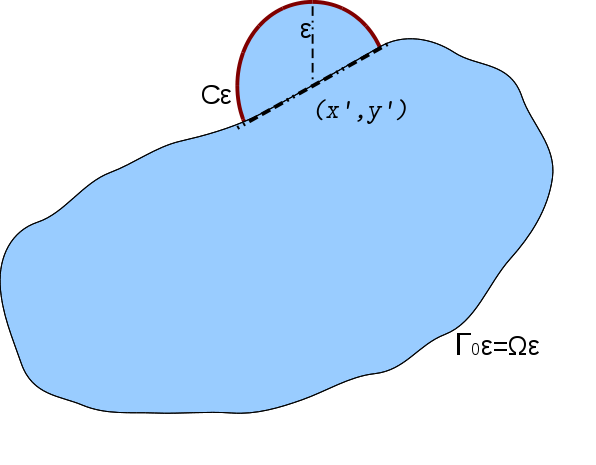
\includegraphics[height = 6cm]{lingkaran2.png}
\end{center}
 \caption{Domain to Avoid Singularity}\label{obstacleEpsilon}
\end{figure}

Let us approximate the integral on $\Gamma_0$ with an integral on $\Gamma_0^\varepsilon$
with $\varepsilon >0$.
From the Figure \ref{obstacleEpsilon}, as $\varepsilon\to0$, we expect $\integ{{\Gamma_0}^\varepsilon=\Omega_\varepsilon}{}{(\cdot)}\to\integ{\Gamma_0}{}{(\cdot)}$.
We know how to compute $\integ{{\Gamma_0}^\varepsilon=\Omega_\varepsilon}{}{(\cdot)}$, there are no singularities.

Let we calculate the Boundary Integral Formulation on the boundary. If $(x',y')\in \Gamma_0$, let we multiply equation
\eqref{problem5} by $G_{x',y'} $ and integrate it over $\Omega_\varepsilon$.
\begin{align}
\integ{\Omega_\varepsilon}{}{ \Delta \psi(x,y) G_{x',y'}(x,y)}=0\\
\integ{\partial\Omega_\varepsilon}{}{(G_{x',y'}\nabla \psi \cdot n) }-
\left\{\integ{\partial\Omega_\varepsilon}{}{\psi \nabla G_{x',y'}(x,y)\cdot n }-
\integ{\Omega_\varepsilon}{}{\psi (x,y)\Delta G_{x',y'}(x,y) }\right\}=0 \\
-\integ{\partial\Omega_\varepsilon}{}{G_{x',y'}u_0 n_x}-\integ{\partial\Omega_\varepsilon}{}{\psi \nabla G_{x',y'}\cdot n}+0=0\\
\integ{\partial\Omega_\varepsilon}{}{u_0 G_{x',y'}n_x+\psi \nabla G_{x',y'}\cdot n} =0 \label{BIboundary}
\end{align}

Let us examine $\integ{\partial\Omega_\varepsilon}{}{u_0 G_{x',y'}n_x+\psi \nabla G_{x',y'}\cdot n}$ as $\varepsilon\to0$
\begin{equation}
 \integ{\partial\Omega_\varepsilon}{}{u_0 G_{x',y'}n_x+\psi \nabla G_{x',y'}\cdot n}=
 \integ{C_\varepsilon}{}{u_0 G_{x',y'}n_x+\psi \nabla G_{x',y'}\cdot n}+
 \integ{\partial\Omega_\varepsilon\setminus C_\varepsilon}{}{u_0 G_{x',y'}n_x+\psi \nabla G_{x',y'}\cdot n}
\end{equation}
When $\varepsilon\to0$, if $\integ{\partial\Omega_\varepsilon\setminus C_\varepsilon}{}{u_0 G_{x',y'}n_x+\psi \nabla G_{x',y'}\cdot n}$ has a limit, then it is called The cauchy Principal Value. 
We denote it $\displaystyle\fpint{\partial\Omega}{}{u_0 G_{x',y'}n_x+\psi \nabla G_{x',y'}\cdot n}$.

let us examine $\integ{C_\varepsilon}{}{u_0 G_{x',y'}n_x+\psi \nabla G_{x',y'}\cdot n}$ as $\varepsilon\to0$.
\begin{align}
\integ{C_\varepsilon}{}{u_0 G_{x',y'}n_x+\psi \nabla G_{x',y'}\cdot n}
=& \integ{\theta^\ast}{\theta^\ast+\pi}{\left\{ \dfrac{1}{2\pi}\ln(\varepsilon) u_0 n_x+\psi \dfrac{1}{2\pi} \dfrac{1}{\varepsilon}\right\}\varepsilon \, d\theta }\\
=& \dfrac{1}{2\pi}\varepsilon\ln{\varepsilon}\integ{\theta^\ast}{\theta^\ast+\pi}{u_0 n_x \, d\theta}
+ \integ{\theta^\ast}{\theta^\ast+\pi}{\dfrac{1}{2\pi}\psi \, d\theta}\\
=&\integ{\theta^\ast}{\theta^\ast+\pi}{\dfrac{1}{2\pi}\psi \, d\theta}\\
=&\dfrac{1}{2\pi}\psi \integ{\theta^\ast}{\theta^\ast+\pi}{\, d\theta}\\
=& \dfrac{1}{2}\psi(x',y') \label{residual}
\end{align}
Result from~\eqref{residual} is called a ``Residual Term''.

Now, we can compute~\eqref{BIboundary} when $\varepsilon\to0$ as follows:
\begin{align}
 \integ{\partial\Omega_\varepsilon}{}{u_0 G_{x',y'}n_x+\psi \nabla G_{x',y'}\cdot n}&=0\\
\fpint{\partial\Omega}{}{u_0 G_{x',y'}n_x+\psi \nabla G_{x',y'}\cdot n}+\dfrac{1}{2\pi}\psi(x',y')&=0\\
\dfrac{1}{2}\psi(x',y')=-\fpint{\partial\Omega}{}{u_0 G_{x',y'}n_x+\psi \nabla G_{x',y'}\cdot n}\label{BIboundary1}
\end{align}
We can calculate boundary integral formulation in equation \eqref{BIboundary1} with numerical method.

\section{Numerical Methods}
\subsection{Solving Boundary Integral Formulation on an Obstacle}

We want to solve numerically Boundary Integral Formulation on the ostacle as we get in equation~\eqref{BIboundary1}. 
First, we consider that on the boundary of obstacle, we have $N$ partitions. Each partition become a straight line $S_i , i= 1,2, \cdots N$, from $(x_i^-,y_i^-)$ to $(x_i^+,y_i^+)$. 
Next, we simply write $(x_i^-,y_i^-)$ and $(x_i^+,y_i^+)$ as $(x^-,y^-)$ and $(x^+,y^+)$ respectively for each partition $i$. We denote $(x_i,y_i)$ be the point in the middle of $S_i$, 
so that it has same length either from $(x^-,y^-)$ or from $(x^+,y^+)$. For ilustration, see figure \ref{sourcePosition}. In figure \ref{sourcePosition}, the point $(x',y')$ is called the source.
For solving boundary integral formulation on the boundary, this source is $(x_i,y_i)$ itself.

In each partition $i$, we have we have the value $\psi_i=\psi(x_i,y_i)$. We can define normal vector in each partition with direction depend on the location where the source is located.
In figure \ref{sourcePosition} we can see that for source $(x',y')$, the direction of normal vector can be different depend on the position of which partition that concern us.

We denote
 \[ e_i(x,y) = \left\{
  \begin{array}{l l}
    1 & \quad \text{if $(x,y)\in S_i$ }\\
    0 & \quad \text{otherwise}
  \end{array} \right.\]
We obtain the value of $\psi$ in obstacle as
\begin{equation}
 \psi(x,y)=\sum\limits_{i=1}^N \psi_i e_i(x,y)
\end{equation}

\begin{figure}[!htbp]
\begin{center}
\includegraphics[height = 4.5 cm]{sourcePosition.eps}
\end{center}
 \caption{source position to the partitions of obstacle}\label{sourcePosition}
\end{figure}

On the obstacle, for $i$ from 1 to $N$ we can write~\eqref{BIboundary1} as 
\begin{align}
 \underbrace{\dfrac{1}{2\pi}\psi(x_i,y_i)}_\text{1} + 
   \underbrace{\fpint{\partial\Omega}{}{\psi \nabla G_{x_i,y_i}\cdot n}}_\text{2}=\underbrace{-\fpint{\partial\Omega}{}{G_{x_i,y_i}u_0n_x}}_\text{3} \label{BIboundary2}
\end{align}
Let us see each item:
\begin{enumerate}
 \item $ \dfrac{1}{2\pi}\psi(x_i,y_i) = \dfrac{1}{2\pi}\psi_i$  

 \item $\displaystyle\fpint{\partial\Omega}{}{\psi \nabla G_{x_i,y_i}\cdot n}=\displaystyle\fpint{\partial\Omega}{}{\left\{\sum\limits_{j=1}^N \psi_j e_j\right\} \nabla G_{x_i,y_i}\cdot n}$
 \begin{align}
\fpint{\partial\Omega}{}{\psi \nabla G_{x_i,y_i}\cdot n}&=\fpint{\partial\Omega}{}{\left\{\sum\limits_{j=1}^N \psi_j e_j\right\} \nabla G_{x_i,y_i}\cdot n}\\
&=\fpint{\partial\Omega}{}{\left\{\sum\limits_{j=1}^N \psi_j e_j\nabla G_{x_i,y_i}\cdot n\right\} }\\
&= \sum\limits_{j=1}^N \left\{ \displaystyle\fpint{\partial\Omega}{}{\psi_je_j\nabla G_{x_i,y_i}\cdot n } \right\}\\
&=\sum\limits_{j=1}^N \psi_j \left\{ \displaystyle\fpint{\partial\Omega}{}{\nabla G_{x_i,y_i}\cdot n e_j} \right\}\\
&=\sum\limits_{j=1}^N\psi_j \left\{ \fpint{S_j}{}{\nabla G_{x_i,y_i}\cdot n} \right\}\\
&=\sum\limits_{j=1}^N \psi_j m_{ij}=(M\psi)_i
\end{align}
with $
      M=(m_{ij})_{\substack{i=1 \cdots N \\j=1 \cdots N}}
     $
and
$
\psi=(\psi_j)_{j=1,\cdots,N}
$. The value $m_{ij}$ is given by the value of integration over $j^{\text{th}}$ line partition $S_j$ with the source is at $(x_i,y_i)$. Then we can write it as $\displaystyle \fpint{S_j}{}{\nabla G_{x_i,y_i}\cdot n}$.

\item $-\displaystyle \fpint{\partial\Omega}{}{G_{x_i,y_i}u_0n_x}$

Since the domain is divided in line, we have $n=\left( \begin{array}{c}
      n_x \\
      n_y
    \end{array}\right)$
and $n_x=\sum\limits_{i=1}^N n_{x_i}e_i$,  $n_y=\sum\limits_{i=1}^N n_{y_i}e_i$.

\begin{align}
-\fpint{\partial\Omega}{}{G_{x_i,y_i} u_0 n_x} &= -u_0 \fpint{\partial\Omega}{}{G_{x_i,y_i} n_x} =
-u_0 \fpint{\partial\Omega}{}{G_{x_i,y_i} \sum\limits_{j=1}^N n_{x_j}e_j}\\
&= -u_0 \fpint{\partial\Omega}{}{\sum\limits_{j=1}^N n_{x_j}e_j G_{x_i,y_i}}\\
&= -u_0\sum\limits_{j=1}^N \fpint{\partial\Omega}{}{n_{x_j}e_j G_{x_i,y_i}}\\
&= -u_0\sum\limits_{j=1}^N n_{x_j} \fpint{\partial\Omega}{}{G_{x_i,y_i}e_j}\\
&=-u_0 \sum\limits_{j=1}^N n_{x_j} \integ{S_j}{}{G_{x_i,y_i}}\\
&=-u_0 (P N_x)_i
\end{align}
with $
      P=(p_{ij})_{\substack{i=1 \cdots N \\j=1 \cdots N}}
     $.
The value $p_{ij}$ is given by the value of integration over $j^{\text{th}}$ line partition $S_j$ with the source is at $(x_i,y_i)$. Then we can write it as $\displaystyle \fpint{S_j}{}{ G_{x_i,y_i}}$.

\end{enumerate}

Furthermore, we will compute $p_{i,j}=\integ{S_j}{}{G_{x_i,y_i}}$ and $m_{i,j}=\displaystyle \fpint{S_j}{}{\nabla G_{x_i,y_i}\cdot n}$ which the calculation process divides in two cases.
\begin{enumerate}
 \item $i\neq j$

Let we see the point $(x',y')$ towards the other points in partition, such in figure \ref{sourcePosition}. If we have $(x_i,y_i)$ on the obstacle as the source, we simply change $(x',y')$ with $(x_i,y_i)$. 

To compute the integral, let us recall the Green function $G$ as in equation \eqref{GreenFunction}:
\[
 G_{x',y'}(x,y)=\dfrac{1}{2 \pi} \, \ln(\sqrt{(x-x')^2+(y-y')^2})
\]
From here we can obtain:
\begin{align}
 \partial_x G_{x',y'}(x,y)=-\dfrac{1}{2 \pi} \, \frac{x-x'}{(x-x')^2+(y-y')^2}\\
 \partial_y G_{x',y'}(x,y)=-\dfrac{1}{2 \pi} \, \frac{y-y'}{(x-x')^2+(y-y')^2}\\
 \nabla G_{x',y'} \cdot n =\dfrac{1}{2 \pi} \frac{(x-x')n_x+(y-y')n_y}{(x-x')^2+(y-y')^2}
\end{align}

Since $\nabla G_{x',y'}$ and $G_{x',y'}$ are radial functions, we can turn the axis in such a way more convenient to examine. 
We notice the position between the source $(x',y')$ and one partition of obstacle in figure \ref{turnAxis1}.
we change the coordinate $xy$ with $\eta \nu$. Coordinate $\eta \nu$ formed by rotation $xy$ coordinate through $\alpha$. 
\begin{figure}[!htbp]
\begin{center}
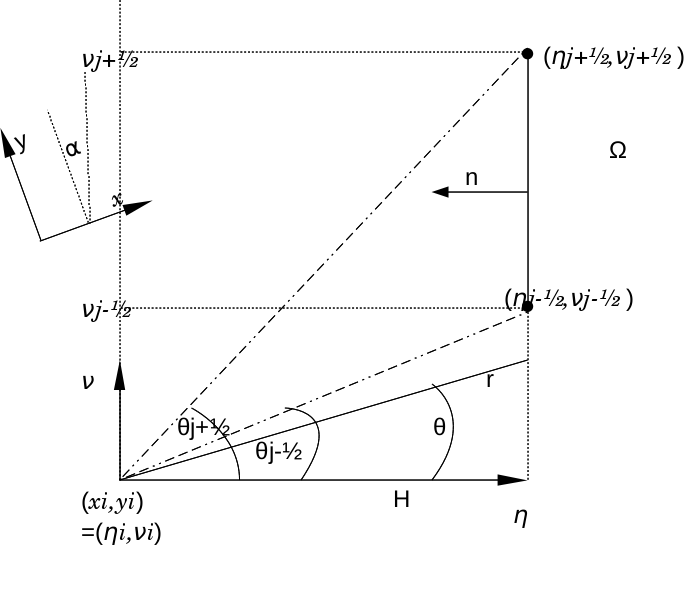
\includegraphics[height = 5.3cm]{changeAxis1.eps}
\end{center}
 \caption{Change the axis and ordinat}\label{turnAxis1}
\end{figure}

In new reference frame, We can write $\eta \nu$ as:
\begin{align}
 \left(\begin{array}{c}
     \eta\\
      \nu 
    \end{array}\right)=& \left( \begin{array}{cc} \cos \alpha & -\sin \alpha \\
           \sin \alpha & \cos \alpha \end{array} \right)
 \left(\begin{array}{c}
     x-x' \\
     y-y'
    \end{array}\right)\\
=& R(\alpha)\left(\begin{array}{c}
     x-x' \\
     y-y'
    \end{array}\right)
\end{align}

\begin{align}
  \eta&=\cos\alpha (x'-x)- \sin \alpha (y-y')\\
\nu&=\sin \alpha(x'-x)+\cos \alpha (y-y')\\
\eta^2+\nu^2=&\left(\begin{array}{c}
     \nu \\
      \eta
    \end{array}\right) \cdot \left(\begin{array}{c}
     \nu \\
      \eta
    \end{array}\right)=\left(\begin{array}{c}
     \nu \\
      \eta
    \end{array}\right)^t \left(\begin{array}{c}
     \nu \\
      \eta
    \end{array}\right)\\
=&\left(R(\alpha)\left(\begin{array}{c}
     x-x' \\
     y-y'
    \end{array}\right)\right)^t \left(R(\alpha)\left(\begin{array}{c}
     x-x' \\
     y-y'
    \end{array}\right)\right)\\
=& \left(\begin{array}{c}
     x-x' \\
     y-y'
    \end{array}\right)^t R^t(\alpha)R(\alpha)\left(\begin{array}{c}
     x-x' \\
     y-y'
    \end{array}\right)\\
=&\left(\begin{array}{c}
     x-x' \\
     y-y'
    \end{array}\right)^t \left(\begin{array}{c}
     x-x' \\
     y-y'
    \end{array}\right)=(x-x')^2+(y-y')^2 \label{kesamaanJarak}
\end{align}

In $\eta \nu$ coordinate, we can use \ref{kesamaanJarak} to write Green function $G$ as
\begin{equation}
  G_{x_i,y_i}(x,y)=\tilde{G}(\eta,\nu)=\frac{1}{2\pi} \ln\left(\sqrt{\eta^2 + \nu^2}\right)
\end{equation}
we can also write $\eta$ and $\nu$ in radial coordinates. Let we say $H$ be a distance between source $(x',y')$ and the partition in $\eta$ coordinate, 
 $\theta^+$ is the angle that formed by $r^+$ and $\eta$ and $\theta^-$ is the angle that formed by $r^-$ and $\eta$. 
\begin{align}
 \eta=r \cos\theta=H\\
\nu=r \sin\theta\\
\frac{\nu}{\eta}=\tan \theta \Leftrightarrow \nu=\eta \tan \theta
\end{align}
Along the integration line $S$ at $\eta=H$, 
\begin{equation}
  \nu=H\tan\theta\Leftrightarrow d\nu=H \frac{1}{\cos^2\theta}= H \sec^2\theta d\theta.
\end{equation}
With using these values, we can get
\begin{align}
\fpint{S}{}{G_{x',y'}}&=\fpint{\nu^-}{\nu^+}{\frac{1}{2\pi}\ln\left(\sqrt{\eta^2 + \nu^2}\right) \, d\nu}\\
&=\fpint{\theta^-}{\theta^+}{\frac{1}{2\pi} 
\left( \ln(r) H \sec^2\theta \right)  \, d\theta}\\
&=\frac{H}{2\pi} \fpint{\theta^-}{\theta^+}{\ln(H\sec\theta) H \sec^2\theta \mathrm{d}\theta}\\
&=\frac{H}{2\pi}\left [ \tan \theta \ln (H\sec\theta)+\theta-\tan\theta \right ]_{\theta^-}^{\theta^+}\label{pij}
\end{align}
From equation \eqref{pij}, we can build the matrix $P=(p_{ij})$ with $p_{ij}= \fpint{S_j}{}{G_{x_i,y_i}}$.

Further, we want to compute $m_{ij}$. First we need the value of $\nabla G_{x',y'}\cdot n$ in $\eta \nu$ coordinate. When the direction of normal vector is equal to direction of $-\eta$, we obtain:
\begin{align}
 \nabla G_{x',y'}\cdot n&=\left(\begin{array}{c}
      \partial_x G_{x',y'}\\
      \partial_y G_{x',y'}
    \end{array}\right) \cdot \left(\begin{array}{c}
      n_x \\
      n_y
    \end{array}\right)\\
&=\left(\begin{array}{c}
      \frac{1}{2\pi} \frac{x-x'}{(x-x')^2+(y-y')^2} \\
      \frac{1}{2\pi} \frac{y-y'}{(x-x')^2+(y-y')^2}
    \end{array}\right) \cdot \left(\begin{array}{c}
      n_x \\
      n_y
    \end{array}\right)\\
&= \frac{1}{2\pi \left((x-x')^2+(y-y')^2 \right)}\left(\begin{array}{c}
     x-x' \\
     y-y'
    \end{array}\right)\cdot \left(\begin{array}{c}
      n_x \\
      n_y
    \end{array}\right)\\
&= \frac{1}{2\pi \left((x-x')^2+(y-y')^2 \right)}\left(\begin{array}{c}
     x-x' \\
     y-y'
    \end{array}\right)\cdot \vec{n}\\
&=\frac{1}{2\pi \left((\eta)^2+(\nu)^2 \right)} \left(\left(R^{-1}(\alpha)\left(\begin{array}{c}
     \eta \\
     \nu
    \end{array}\right)\right)\cdot \vec{n}\right)\\
=& \frac{1}{2\pi \left((\eta)^2+(\nu)^2 \right)} \left(\left(R(-\alpha)\left(\begin{array}{c}
     \eta \\
     \nu
    \end{array}\right)\right)\cdot \vec{n}\right)\\
=&\frac{1}{2\pi \left((\eta)^2+(\nu)^2 \right)}\left(\left(\begin{array}{c}
     \eta \\
     \nu
    \end{array}\right)\cdot R^{t}(-\alpha) \vec{n}\right)\\
&=\frac{1}{2\pi \left((\eta)^2+(\nu)^2 \right)} \left( \left(\begin{array}{c}
     \eta \\
     \nu
    \end{array} \right) \cdot R(\alpha) \vec{n}\right)\\
=&\frac{1}{2\pi \left((\eta)^2+(\nu)^2 \right)} \left(\left(\begin{array}{c}
     \eta \\
     \nu
    \end{array}\right) \cdot \left(\begin{array}{c}
      -1 \\
      0
    \end{array}\right)\right)\\
&=\frac{-\eta}{2\pi \left((\eta)^2+(\nu)^2 \right)}
\end{align}
With the similar calculation, when the normal vector is in the same direction with $\eta$, we get:
\begin{equation}
 \nabla G_{x',y'}\cdot n=\frac{\eta}{2\pi \left((\eta)^2+(\nu)^2 \right)} 
\end{equation}
So that
\begin{equation}
  \nabla G_{x',y'}\cdot n=s\frac{\eta}{2\pi \left((\eta)^2+(\nu)^2 \right)}\label{NablaGnRadial}
\end{equation}
With
\[
 s=\left\{ \begin{array}{ll}
    -1, & \text{ if direction } n \text{ is equal to }-\eta\\
    1, & \text{ if direction } n \text{ is equal to } \eta
   \end{array}\right.
\]

From equation \ref{NablaGnRadial}, we get
\begin{align}
\fpint{S}{}{\nabla G{x',y'}\cdot n}&=\fpint{\nu^-}{\nu^+}{\frac{s}{2\pi} \frac{\eta}{\eta^2+\nu^2} \, d\nu}\\
&=\fpint{\theta^-}{\theta^+}{\frac{sH}{2\pi H^2\sec^2\theta}H \sec^2\theta \, d\theta}\\
&= \frac{s}{2\pi} \fpint{\theta^-}{\theta^+}{\, d\theta}\\
&=\frac{s}{2\pi}(\theta^+ - \theta^-)
\end{align}

 \item $i=j$

 We can see in figure \ref{iEqualj} when $i=j$ in $\eta\nu$ coordinate. The source $(x',y')=(x_i,y_i)$ is located in the middle of $(x^+,y^+)$ and $(x^-,y^-)$. Let us suppose $l_i$ as distance between $\nu^+$ and $\nu^-$. 
\begin{figure}[!htbp]
\begin{center}
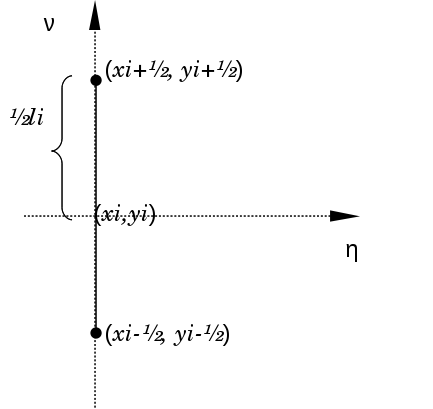
\includegraphics[height = 6cm]{iEqualj.eps}
\end{center}
 \caption{Position when i equal to j}\label{iEqualj}
\end{figure}
Hence, we obtain:
\begin{align}
\fpint{S}{}{G_{x',y'}}=&\lim_{\varepsilon \to 0} \integ{\nu^-}{-\varepsilon}{G_{x',y'}(0,\nu) \, d\nu} + \integ{\varepsilon}{\nu^+}{G_{x',y'}(0,\nu) \, d\nu}\\
 =&\lim_{\varepsilon \to 0} \integ{\nu^-}{-\varepsilon}{\frac{1}{2\pi}\ln \left( \sqrt{0 + \nu^2}\right) \, d\nu}+
 \integ{\varepsilon}{\nu^+}{\frac{1}{2\pi}\ln \left( \sqrt{0 + \nu^2}\right) \, d\nu}\\ 
   =&\lim_{\varepsilon \to 0} \integ{-\frac{l_i}{2}}{-\varepsilon}{\frac{1}{2\pi}\ln\left( \lvert \nu \rvert \right) \, d\nu}+ 
 \integ{\varepsilon}{\frac{l_i}{2}}{\frac{1}{2\pi} \ln\left( \lvert \nu \rvert \right) \, d\nu}\\
 =&\frac{2}{2\pi} \lim_{\varepsilon \to 0} \integ{\varepsilon}{\frac{l_i}{2}}{\frac{1}{2\pi}\ln \left( \nu \right) \, d\nu}\\
 =&\frac{1}{\pi} \lim_{\varepsilon \to 0} \left(\nu \ln\nu-\nu \right)_\varepsilon^{\frac{l_i}{2}}\\
 =&\frac{1}{\pi} \lim_{\varepsilon \to 0} \left\{ \left( \frac{l_i}{2}\ln \left( \frac{l_i}{2} \right)-\frac{l_i}{2} \right)- \left( \varepsilon \ln\varepsilon- \varepsilon \right) \right\}\\
=& \frac{1}{\pi} \left( \frac{l_i}{2}\ln \left( \frac{l_i}{2} \right)-\frac{l_i}{2} \right)
 \end{align}
 
 As long as $G$ is a radial function, $\nabla G$ is also radial (radial vector). Using equation \eqref{NablaGnRadial}, we get 
\begin{align}
 \fpint{S}{}{\nabla G{x',y'}\cdot n} &=\lim_{\varepsilon \to 0} \integ{-\frac{l_i}{2}}{-\varepsilon}{\nabla G{x',y'}\cdot n (0,\nu)\, d\nu}+ \integ{\varepsilon}{\frac{l_i}{2}}{\nabla G{x',y'}\cdot n (0,\nu) \, d\nu}\\
 &=0
\end{align}
 
\end{enumerate}

From the calculation above, we can write~\eqref{BIboundary2} as following equation system:
\begin{equation}\label{SPL}
 \left( \frac{1}{2} I+M \right) \psi= -u_0 P N_x 
\end{equation}
with 
\[  m_{ij}= \left\{
  \begin{array}{l l}
    0 & \quad \text{if $i=j$ }\\
    \frac{s}{2\pi}(\theta^+-\theta^-) & \quad \text{otherwise}
  \end{array} \right.,\]
   \[
 s=\left\{ \begin{array}{ll}
    -1, & \text{ if direction } n \text{ is equal to }-\eta\\
    1, & \text{ if direction } n \text{ is equal to } \eta
   \end{array}\right.
\]
  and
  \[  p_{ij}= \left\{
  \begin{array}{l l}
     \frac{1}{\pi} \left( \frac{l_i}{2}\ln \left( \frac{l_i}{2} \right)-\frac{l_i}{2} \right) & \quad \text{if $i=j$ }\\
    \frac{H}{2\pi}\left [ \tan \theta \ln (H\sec\theta)+\theta-\tan\theta \right ]_{\theta^-}^{\theta^+} & \quad \text{otherwise}
  \end{array} \right.\]

  
\subsection{Solving Boundary Integral Formulation in Domain}

We want to solve the boundary integral formulation when the source is in the domain $(x',y')\in \Omega$ as in equation~\eqref{BIform}. 
\begin{equation}
 \psi(x',y')=-\integ{\Gamma_0}{}{(-u_0 n_x)G_{x',y'}(x,y)} + \integ{\Gamma_0}{}{\psi\nabla G_{x',y'}(x,y)\cdot \vec{n}} \label{BIform1}
\end{equation}
If we call $-u_0 n_x$ and $\psi$ respectively with Neum and Diri, we can write \ref{BIform1} as
\begin{equation}
 \psi(x',y')=-\integ{\Gamma_0}{}{\text{Neum}G_{x',y'}(x,y)} + \integ{\Gamma_0}{}{\text{Diri}\nabla G_{x',y'}(x,y)\cdot \vec{n}}
\end{equation}

For solving Boundary Integral Formulation inside the domain, in order to get the potential flow, we wish to obtain $u=\nabla\psi$ as in equation \eqref{Pr0}.
\begin{equation}
 \nabla\psi=\left(\begin{array}{c}
      \partial_{x'}\psi \\
      \partial_{y'}\psi
    \end{array}\right) \label{nablaPsi}
\end{equation}
First, let we compute $\partial_{x'}\psi$ and $\partial_{y'}\psi$.
\begin{align}
 \partial_{x'}\psi(x',y')&=\partial_{x'}\left(-\integ{\Gamma_0}{}{\text{Neum}G_{x',y'}(x,y)} + \integ{\Gamma_0}{}{\text{Diri}\nabla G_{x',y'}(x,y)\cdot \vec{n}} \right)\\
&=  \underbrace{-\integ{\Gamma_0}{}{\text{Neum} \left(\partial_{x'}G_{x',y'}(x,y)\right)}}_\text{1}  +  
\underbrace{\integ{\Gamma_0}{}{\text{Diri}\left(\partial_{x'}\nabla G_{x',y'}(x,y)\cdot \vec{n}\right)}}_\text{2}\label{partialxaPsi} 
\end{align}
\begin{align}
 \partial_{y'}\psi(x',y')&=  \underbrace{-\integ{\Gamma_0}{}{\text{Neum} \left(\partial_{y'}G_{x',y'}(x,y)\right)}}_\text{3}  +  
\underbrace{\integ{\Gamma_0}{}{\text{Diri}\left(\partial_{y'}\nabla G_{x',y'}(x,y)\cdot \vec{n}\right)}}_\text{4} \label{partialyaPsi}
\end{align}

We use Green function as in equation \ref{GreenFunction}. We obtain:
\begin{align}
 \partial_{x'} G_{x',y'}(x,y)=-\frac{1}{2\pi}\frac{x-x'}{(x-x')^2+(y-y')^2}\\ \label{partialxaG}
\partial_{y'} G_{x',y'}(x,y)=-\frac{1}{2\pi}\frac{y-y'}{(x-x')^2+(y-y')^2} \\ \label{partialyaG}
\nabla G_{x',y'} \cdot n= \frac{1}{2\pi} \frac{(x-x')n_x+(y-y')n_y}{(x-x')^2+(y-y')^2}
\end{align}
\begin{align}
 \partial_{x'}\nabla G_{x',y'} \cdot n &=\frac{1}{2\pi} \frac{(-n_x)((x-x')^2+(y-y')^2)-(-2(x-x')(n_x(x-x')+n_y(y-y')))}{((x-x')^2+(y-y')^2)^2}\\
&= -\frac{1}{2\pi}  \frac{(n_x)((x-x')^2+(y-y')^2)-(2(x-x')(n_x(x-x')+n_y(y-y')))}{((x-x')^2+(y-y')^2)^2} \label{partialxaNablaGn}
\end{align}
\begin{align}
 \partial_{y'}\nabla G_{x',y'} \cdot n =-\frac{1}{2\pi}  \frac{(n_y)((x-x')^2+(y-y')^2)-(2(y-y')(n_x(x-x')+n_y(y-y')))}{((x-x')^2+(y-y')^2)^2}\label{partialyaNablaGn}
\end{align}

We can see position $(x',y')$ towards partitions of obstacle as in figure \ref{sourcePosition}. Because $G$ and $\nabla G$ are radial functions,
we can turn the axis and ordinat in such a convenient way as before. See in figure \ref{turnAxis1}. 

We can also write every point in  $\eta\nu$ coordinate as rotation of $xy$. When direction of normal vector is equal to direction $\eta$, we have:
\begin{equation}
\left(\begin{array}{c}
      x-x' \\
      y-y'
    \end{array}\right)=\left(\begin{array}{cc}
      n_x & -n_y \\
      n_y & n_x
    \end{array}\right)\left(\begin{array}{c}
      \eta\\
      \nu
    \end{array}\right) \label{RotasixNu}
\end{equation}

Moreover, if direction of normal vector is equal to $-\eta$, we hold
\begin{equation}
\left(\begin{array}{c}
      x-x' \\
      y-y'
    \end{array}\right)=\left(\begin{array}{cc}
      -n_x & n_y \\
      -n_y & -n_x
    \end{array}\right)\left(\begin{array}{c}
      \eta\\
      \nu
    \end{array}\right) \label{RotasixNu1}.
\end{equation}



Furthermore, to calculate potential flow at all points in domain, we need to compute 1, 2, 3 and 4.
\begin{enumerate}
 \item We have to find the value of $-\integ{\Gamma_0}{}{\partial_{x'} G_{x',y'} \text{Neum}}$

 \begin{align}
  -\integ{\Gamma_0}{}{\partial_{x'} G_{x',y'} \text{Neum}}&=-\sum\limits_{i=1}^N  \integ{S_i}{}{\partial_{x'} G_{x',y'} \text{Neum}}\\
  &=-\sum\limits_{i=1}^N \text{Neum}_i \integ{S_i}{}{\partial_{x'} G_{x',y'}}
 \end{align}

Using \eqref{partialxaG} at $x'=x_i$ and equation \eqref{RotasixNu}, when normal vector in the same direction with $\eta$ , let us compute the integral
\begin{align}
 \integ{S_i}{}{\partial_{x'} G_{x',y'}} &= \integ{S_i}{}{-\frac{1}{2\pi}\frac{x-x'}{(x-x')^2+(y-y')^2}}\\
 &=\integ{\nu^+}{\nu^-}{-\frac{1}{2\pi} \frac{n_x\eta-n_y \nu}{\eta^2+\nu^2} \, d\nu}\\
 &=-\frac{1}{2\pi} \integ{\theta^+}{\theta^-}{\frac{H n_x-n_y r \sin\theta}{\left( H\sec\theta\right)^2 }H \sec^2\theta \, d\theta}\\
&=-\frac{1}{2\pi} \integ{\theta^+}{\theta^-}{(n_x-n_y\tan\theta) \, d\theta}\\
&=-\frac{1}{2\pi} \left(\left[ n_x(\theta) + n_y \ln(\vert \cos\theta\vert )\right]_{\theta^+}^{\theta^-} \right)\\
&= \frac{1}{2\pi} \left(\left[ n_x(\theta) + n_y \ln(\vert \cos\theta\vert )\right]_{\theta^-}^{\theta^+} \right)\label{intPartialxaG} 
\end{align}
When direction of normal vector is $-\eta$, we calculate the integral in similar way as above. We get:
\begin{align}
 \integ{S_i}{}{\partial_{x'} G_{x',y'}} &= \integ{S_i}{}{-\frac{1}{2\pi}\frac{x-x'}{(x-x')^2+(y-y')^2}}\\
 &=\integ{\nu^-}{\nu^+}{-\frac{1}{2\pi} \frac{-n_x\eta+n_y \nu}{\eta^2+\nu^2} \, d\nu}\\
 &=-\frac{1}{2\pi} \integ{\theta^-}{\theta^+}{\frac{-H n_x+n_y r \sin\theta}{\left( H\sec\theta\right)^2 }H \sec^2\theta \, d\theta}\\
&=-\frac{1}{2\pi} \integ{\theta^-}{\theta^+}{(-n_x+n_y\tan\theta) \, d\theta}\\
&= -\frac{1}{2\pi} \left(\left[ -n_x(\theta) - n_y \ln(\vert \cos\theta\vert )\right]_{\theta^-}^{\theta^+} \right)\\
&= \frac{1}{2\pi} \left(\left[ n_x(\theta) + n_y \ln(\vert \cos\theta\vert )\right]_{\theta^-}^{\theta^+} \right)
\end{align}
From the calculation above, we obtain:
\begin{equation}
 -\integ{\Gamma_0}{}{\partial_{x'} G_{x',y'} \text{Neum}}=-\sum\limits_{i=1}^N \frac{\text{Neum}_i}{2\pi} \left( \left[ n_x(\theta) + n_y \ln(\vert \cos\theta\vert )\right]_{\theta^-}^{\theta^+} \right) 
\end{equation}

\item We have to compute $\integ{\Gamma_0}{}{\partial_{x'}\nabla G_{x',y'} \cdot n \text{diri}}$

\begin{align}
  \integ{\Gamma_0}{}{\partial_{x'}\nabla G_{x',y'} \cdot n \text{diri}}=\sum\limits_{i=1}^N \text{diri}_i \integ{\Gamma_0}{}{\partial_{x'}\nabla G_{x',y'} \cdot n}
\end{align}
With using equation \ref{partialxaNablaGn}, and normal vector in the same direction with $\eta$, we can write:
\begin{align}
 \integ{\Gamma_0}{}{\partial_{x'}\nabla G_{x',y'} \cdot n}&=\integ{\nu^+}{\nu^-}{-\frac{1}{2\pi} \frac{(\eta^2+\nu^2)n_x-2(n_x\eta-n_y\nu)(\eta)}{(\eta^2+\nu^2)^2} \, d\nu}\\
 =& \integ{\theta^+}{\theta^-}{-\frac{1}{2\pi} \frac{(H^2 \sec^2\theta)n_x-2(n_x H-n_y H \sec \theta \sin \theta)(H)}{H^4 \sec^4\theta} \, H \sec^2\theta d\theta}\\
=&\integ{\theta^+}{\theta^-}{-\frac{1}{2\pi} \left( \frac{n_x}{H}-\frac{2n_x}{H \sec^2\theta}+\frac{2n_y \sin \theta \cos\theta}{H} \right) \, d\theta}\\
=&-\frac{1}{2\pi} \left(\frac{n_x}{H} \integ{\theta^+}{\theta^-}{\, d\theta}-
 \frac{n_x}{H} \integ{\theta^+}{\theta^-}{2\cos^2\theta \, d\theta}+
 \frac{n_y}{H} \integ{\theta^+}{\theta^-}{2\cos \theta \sin\theta, d\theta} \right)\\
=& \frac{1}{2\pi} \left[-\frac{n_x}{2H}\sin2\theta+\frac{n_y}{H}\sin^2\theta \right]_{\theta^-}^{\theta^+}\label{intPartialxaNablaGn}
\end{align}
When normal vector has direction $-\eta$, we obtain:
\begin{align}
 \integ{\Gamma_0}{}{\partial_{x'}\nabla G_{x',y'} \cdot n}&= \integ{\nu^-}{\nu^+}{\frac{1}{2\pi} \frac{(\eta^2+\nu^2)(-n_x)+2(-n_x\eta+n_y\nu)(-\eta)}{(\eta^2+\nu^2)^2} \, d\nu}\\
 =& \integ{\theta^-}{\theta^+}{\frac{1}{2\pi} \frac{(H^2 \sec^2\theta)(-n_x)+2(-n_x H+n_y H \sec \theta \sin \theta)(-H)}{H^4 \sec^4\theta} \, H \sec^2\theta d\theta}\\
=&\integ{\theta^-}{\theta^+}{\frac{1}{2\pi} \left( \frac{-n_x}{H}+\frac{2n_x}{H \sec^2\theta}-\frac{2n_y \sin \theta \cos\theta}{H} \right) \, d\theta}\\
=&\frac{1}{2\pi} \left(\frac{-n_x}{H} \integ{\theta^-}{\theta^+}{\, d\theta}+
 \frac{n_x}{H} \integ{\theta^-}{\theta^+}{2\cos^2\theta \, d\theta}-
 \frac{n_y}{H} \integ{\theta^-}{\theta^+}{2\cos \theta \sin\theta, d\theta} \right)\\
=& \frac{1}{2\pi} \frac{n_x}{H} \integ{\theta^-}{\theta^+}{\cos 2\theta}-\frac{n_y}{H}\integ{\theta^-}{\theta^+}{2\cos \theta \sin\theta, d\theta}\\
=& \frac{1}{2\pi} \left[\frac{n_x}{2H}\sin2\theta-\frac{n_y}{H}\sin^2\theta-\frac{n_x}{H} 2 \theta \right]_{\theta^-}^{\theta^+}\label{intPartialxaNablaGn1}
\end{align}
From the calculation above, we obtain:
\begin{align}
 \integ{\Gamma_0}{}{\partial_{x'}\nabla G_{x',y'} \cdot n \text{diri}}=\sum\limits_{i=1}^N \text{diri}_i\frac{s}{2\pi} \left[-\frac{n_x}{2H}\sin2\theta+\frac{n_y}{H}\sin^2\theta \right]_{\theta^-}^{\theta^+}
\end{align}
with
 \[
 s=\left\{ \begin{array}{ll}
    -1, & \text{ if direction } n \text{ is equal to }-\eta\\
    1, & \text{ if direction } n \text{ is equal to } \eta
   \end{array}\right.
\]

\item We will calculate $-\integ{\Gamma_0}{}{\text{Neum} \left(\partial_{y'}G_{x',y'}(x,y)\right)}$

\begin{equation}
 -\integ{\Gamma_0}{}{\partial_{y'} G_{x',y'} \text{Neum}}=-\sum\limits_{i=1}^N  \integ{S_i}{}{\partial_{y'} G_{x',y'} \text{Neum} \, dS}
\end{equation}
We use \ref{partialyaG} and \ref{RotasixNu} when normal vector has the same direction with $\eta$, to obtain:

\begin{align}
 \integ{S_i}{}{\partial_{y'} G_{x',y'}}&=\integ{S_i}{}{-\frac{1}{2\pi}\frac{y-y'}{(x-x')^2+(y-y')^2}}\\
 &=\integ{\nu^+}{\nu^-}{-\frac{1}{2\pi} \frac{n_y\eta+n_x \nu}{\eta^2+\nu^2} \, d\nu}\\
&=-\frac{1}{2\pi}\integ{\theta^+}{\theta^-}{\frac{H n_y+n_x r \sin\theta}{\left( H\sec\theta\right)^2 }H \sec^2\theta \, d\theta}\\
&=-\frac{1}{2\pi}\integ{\theta^+}{\theta^-}{n_y+n_x\tan\theta\, d\theta}\\
&=\frac{1}{2\pi} \left[ n_y\theta -n_x \ln(\vert \cos\theta\vert \right]_{\theta^-}^{\theta^+} \label{intPartialyaG1}
\end{align}
When normal vector has direction $-\eta$, we obtain:
\begin{align}
 \integ{S_i}{}{\partial_{y'} G_{x',y'}}&=\integ{S_i}{}{-\frac{1}{2\pi}\frac{y-y'}{(x-x')^2+(y-y')^2}}\\
 &=\integ{\nu^+}{\nu^-}{-\frac{1}{2\pi} \frac{-n_y\eta-n_x \nu}{\eta^2+\nu^2} \, d\nu}\\
&=-\frac{1}{2\pi}\integ{\theta^+}{\theta^-}{\frac{-H n_y-n_x r \sin\theta}{\left( H\sec\theta\right)^2 }H \sec^2\theta \, d\theta}\\
&=-\frac{1}{2\pi}\integ{\theta^+}{\theta^-}{-n_y-n_x\tan\theta\, d\theta}\\
&=\frac{1}{2\pi} \left[ n_y\theta -n_x \ln(\vert \cos\theta\vert \right]_{\theta^-}^{\theta^+} \label{intPartialyaG11}
\end{align}
From the calculation above, we obtain:
\begin{align}
 -\integ{\Gamma_0}{}{\partial_{y'} G_{x',y'} \text{Neum}}=-\sum\limits_{i=1}^N \frac{\text{Neum}_i}{2\pi}\left[ n_y\theta -n_x \ln(\vert \cos\theta\vert \right]_{\theta^-}^{\theta^+} \label{intPartialyaG}
 \end{align}

\item We will find the value of $\integ{\Gamma_0}{}{\text{Diri}\left(\partial_{y'}\nabla G_{x',y'}(x,y)\cdot \vec{n}\right)}$
\[
  \integ{\Gamma_0}{}{\partial_{y'}\nabla G_{x',y'} \cdot n \text{diri}}=\sum\limits_{i=1}^N \text{diri}_i \integ{\Gamma_0}{}{\partial_{y'}\nabla G_{x',y'} \cdot n}
\]
Using equation \ref{partialyaNablaGn} and \ref{RotasixNu} when normal vector has the same direction with $\eta$, we can write:
\begin{align}
 \integ{\Gamma_0}{}{\partial_{y'}\nabla G_{x',y'} \cdot n}
 &= \integ{\nu^+}{\nu^-}{-\frac{1}{2\pi} \frac{(\eta^2+\nu^2)n_y-2(n_y\eta+n_x\nu)(\eta)}{(\eta^2+\nu^2)^2} \, d\nu}\\
&=\integ{\theta^+}{\theta^-}{-\frac{1}{2\pi} \frac{\left((H^2 \sec^2\theta)n_y-2(n_y H+n_x H \sec \theta \sin \theta)(H)\right)H \sec^2\theta}{H^4 \sec^4\theta} \, d\theta}\\
&= \integ{\theta^+}{\theta^-}{-\frac{1}{2\pi} \left( \frac{n_y}{H}-\frac{2n_y}{H \sec^2\theta}-\frac{2n_x \sin \theta \cos\theta}{H} \right) \, d\theta}\\
&= -\frac{1}{2\pi} \left(\frac{n_y}{H} \integ{\theta^+}{\theta^-}{\, d\theta}-
 \frac{n_y}{H} \integ{\theta^+}{\theta^-}{2\cos^2\theta \, d\theta}-
 \frac{n_x}{H} \integ{\theta^+}{\theta^-}{2\cos \theta \sin\theta, d\theta} \right)\\
&= \frac{1}{2\pi} \left[-\frac{n_y}{2H}\left(\sin2\theta\right)-\frac{n_x}{H}\sin^2\theta \right]_{\theta^-}^{\theta^+}\label{intPartialyaNablaGn1}
\end{align}
If normal vector has direction $-\eta$, we obtain:
\begin{align}
 \integ{\Gamma_0}{}{\partial_{y'}\nabla G_{x',y'} \cdot n}
 &= \integ{\nu^-}{\nu^+}{\frac{1}{2\pi} \frac{(\eta^2+\nu^2)-n_y+2(-n_y\eta-n_x\nu)(-\eta)}{(\eta^2+\nu^2)^2} \, d\nu}\\
&=\integ{\theta^-}{\theta^+}{-\frac{1}{2\pi} \frac{\left((H^2 \sec^2\theta)n_y+2(-n_y H-n_x H \sec \theta \sin \theta)(H)\right)H \sec^2\theta}{H^4 \sec^4\theta} \, d\theta}\\
&= \integ{\theta^-}{\theta^+}{-\frac{1}{2\pi} \left( \frac{n_y}{H}-\frac{2n_y}{H \sec^2\theta}-\frac{2n_x \sin \theta \cos\theta}{H} \right) \, d\theta}\\
&= -\frac{1}{2\pi} \left(\frac{n_y}{H} \integ{\theta^-}{\theta^+}{\, d\theta}-
 \frac{n_y}{H} \integ{\theta^-}{\theta^+}-{2\cos^2\theta \, d\theta}-
 \frac{n_x}{H} \integ{\theta^-}{\theta^+}{2\cos \theta \sin\theta, d\theta} \right)\\
&= -\frac{1}{2\pi} \left[-\frac{n_y}{2H} \sin2\theta-\frac{n_x}{H}\sin^2\theta \right]_{\theta^-}^{\theta^+}\label{intPartialyaNablaGn11}
\end{align}

From the calculation above, we obtain:
\begin{equation}
 \integ{\Gamma_0}{}{\partial_{y'}\nabla G_{x',y'} \cdot n \text{diri}}=\sum\limits_{i=1}^N \text{diri}_i\frac{s}{2\pi} \left[-\frac{n_y}{2H}\left(\sin2\theta\right)-\frac{n_x}{H}\sin^2\theta \right]_{\theta^-}^{\theta^+}
\end{equation}
with
 \[
 s=\left\{ \begin{array}{ll}
    -1, & \text{ if direction } n \text{ is equal to }-\eta\\
    1, & \text{ if direction } n \text{ is equal to } \eta
   \end{array}\right.
\]

\end{enumerate}

\end{document}
